%!TEX root = ../main.tex


\section{End-to-end learning approach}
\label{sec:end2endLearning}

The control policy employed in this work is end-to-end: the NN takes as inputs the raw sensor data and directly outputs the control values (steering and throttle in this case). In addition, the policy is trained from scratch. The objective for the navigation algorithm is to control a John Deere Gator to reach a target destination given by GPS coordinates. The algorithm uses a GPS and IMU that provide the neural network with the current vehicle location and orientation. The vehicle is also equipped with a low-resolution RGB camera, which the network includes as input in order to allow for avoiding obstacles (rocks of various shapes, sizes, and textures).

For training, the environment consists of a 120x120 m swath of terrain on which obstacles are placed randomly. The vehicle initial position is picked randomly on a 80 m diameter circle while the goal is placed on the opposite side of the same circle; in other words, given $\alpha$ the angle of the vehicle initial position, the angle of the goal will be $\alpha + \beta$ with $\beta \in [\frac{\pi}{2} , \frac{3\pi}{2}]$.
The vehicle must navigate to within 10 m of the destination and the reward is proportional to the vehicle's approaching speed. The episode is terminated with a reward penalty if the vehicle hits an obstacle, goes outside the terrain boundary, or the timeout is reached, while it is terminated with a reward bonus if it reaches the goal.
The observation consists of a two-element tuple: an 80x45 pixel RGB image and a five-element array containing the components (x,y) of the distance from the goal (in the vehicle frame, based on GPS measurements), the vehicle orientation (compass angle), the heading with respect to the goal, and the vehicle speed. 
Based on these inputs, the policy controls the steering (-1 to 1) and the throttle/brake value (-1 to 1, with negatives implying braking). 
To train the NN, we adopted the constrained version of the Proximal Policy Optimization (PPO) algorithm \cite{Schulman2017PPO}, using two separated NN for the actor and the critic. PPO is known as one of the best performing DRL algorithms for continuous control \cite{openai2018HandManipulation}.
The NN model inputs come from several sensors: GPS, IMU, and RGB camera. Through PyTorch \cite{paszke2017PyTorch} the NN model was implemented as follows. A five-element array is fed to a fully connected layer, while the RGB image is processed by a CNN as in \cite{Mnih13}. The output of the CNN and the single fully connected hidden layer are concatenated and then processed through three fully-connected hidden layers, as shown in Fig. \ref{fig:NN_arch}. All layers use the ReLU activation function.

\begin{figure}[h]
    \centering
    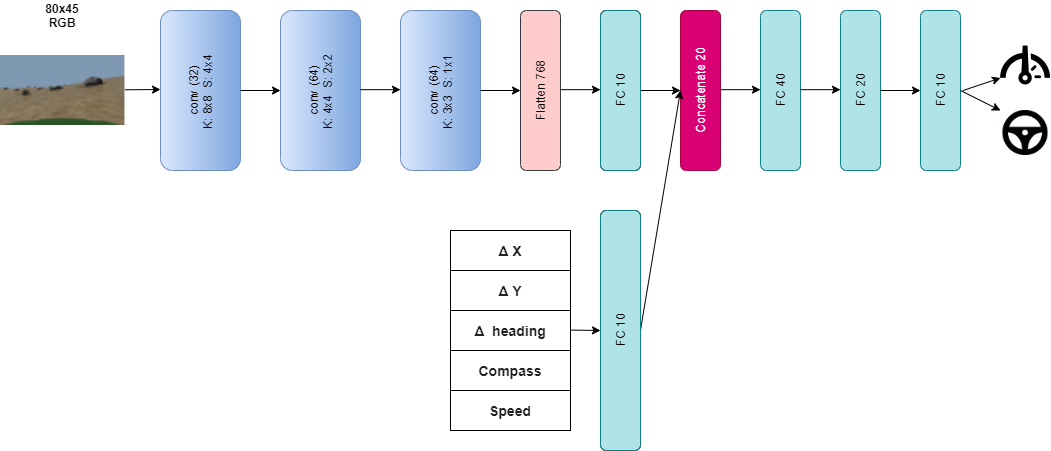
\includegraphics[width=.95\linewidth]{images/CORL_paper_arch.pdf}
    \caption{Actor neural network architecture}
    \label{fig:NN_arch}
\end{figure}


%local vs global (from GPS)


Given the GPS coordinates of the vehicle and the goal, along with the orientation of the vehicle from the IMU, it is straightforward (for a human) to evaluate the distance between the vehicle and the objective. This being said, there are several ways to pass this information to the NN as an input: directly feeding the GPS coordinates, the coordinate difference, the relative distance in a frame oriented along the cardinal points or the distance in the local frame of the vehicle. The last is obviously the most meaningful information but we might want to use coarser inputs and leave to the optimization to infer the correlation. This approach, however, would be inefficient as shown in Fig. \ref{fig:plotLocGlob}, where is clearly shown the benefit, in terms of convergence, of simply rotating the position of the goal with respect to the vehicle in the vehicle reference frame (called \emph{local}).


\begin{wrapfigure}{r}{0.50\textwidth}
    \vspace{-25pt}
    \begin{center}
        \includegraphics[width=.90\linewidth]{images/rewards_localglobal.pdf}
        \caption{On flat terrain without obstacles, the algorithm converges immediately when feeding the position of the goal rotated in the vehicle reference frame. When the position is given in the global frame, training does not converge.}
        \label{fig:plotLocGlob}
    \end{center}
    \vspace{-15pt}
\end{wrapfigure}We adopted a curriculum learning approach \cite{BengioCurriculumLearning09}, progressively increasing the complexity of the task, as shown in Fig. \ref{fig:rew_progr}. The first part of the training was performed on flat terrain with a random number of obstacles (from 0 to 30). After $\sim$ 200 policy updates, when the convergence is reached, the obstacle number is fixed at 30, and after a drop off the convergence is reached again quickly. When, after 376 policy updates, the flat terrain is replaced with hilly terrain (while keeping the same number of obstacles), the agent struggles and many updates are required in order to converge again. In the third and last stage of the training, the obstacle count was increased to 50 and the terrain texture was randomized. Curriculum learning was deemed necessary when convergence could not be directly reached from scratch on hilly terrain. Moving through multiple training approaches, we found that: ($i$) Irregularities in terrain height cause policies trained exclusively on flat terrains to perform poorly; ($ii$) This problem can by solved by undergoing further training on hilly terrain; and, ($iii$) The curriculum learning approach (see Fig.~\ref{fig:rew_progr}) was instrumental in eventually handling the complex tasks; i.e., hills with many random obstacles.


% distributed training, batch and minibatch size, Adam with HP, 
Training relied on the ADAM algorithm \cite{Kingma14ADAM} with a learning rate of 1e-4. The training set at each update included 6000 tuples (timesteps), fed by 1000 element mini-batches to the optimizer, which operated eight epochs per update.
Since Chrono is compatible with OpenAI gym \cite{Brockman16Gym} environments, the dataset was collected by running six parallel episodes leveraging OpenAI baselines \cite{baselines} multiprocessing tools.
% MB size comment?
\begin{figure}[h]
    \centering
    \includegraphics[width=.75\linewidth]{images/CORLrewards.pdf}
    \caption{Reward progression. Vertical lines represent the changes introduced to make the environment more challenging. In order of occurrence, the dotted lines mark: fix obstacle count at 30; change from flat to hilly terrain; and increase of obstacle count to 50. }
    \label{fig:rew_progr}
\end{figure}

